% This is samplepaper.tex, a sample chapter demonstrating the
% LLNCS macro package for Springer Computer Science proceedings;
% Version 2.20 of 2017/10/04
%
\documentclass[runningheads, orivec]{llncs}
%
\usepackage{graphicx}
% Used for displaying a sample figure. If possible, figure files should
% be included in EPS format.
\usepackage{amsmath}
\usepackage{amssymb}
\usepackage{float}
%
% If you use the hyperref package, please uncomment the following line
% to display URLs in blue roman font according to Springer's eBook style:
\usepackage[pagebackref=true,breaklinks=true,letterpaper=true,colorlinks,bookmarks=false]{hyperref}
\renewcommand\UrlFont{\color{blue}\rmfamily}

\begin{document}
%
\title{CALVIS: Chest, wAist and peLVIS circumference from 3D human body meshes	
as ground truth for deep learning}
%
\titlerunning{Chest, wAist and peLVIS circumference from 3D human body meshes}
% If the paper title is too long for the running head, you can set
% an abbreviated paper title here
%
\author{Yansel Gonzalez Tejeda\orcidID{0000-0003-1002-3815} \and
Helmut Mayer\orcidID{1111-2222-3333-4444}}
%
\authorrunning{Gonzalez and Mayer}
% First names are abbreviated in the running head.
% If there are more than two authors, 'et al.' is used.
%
\institute{Paris Lodron University of 
	Salzburg, Kapitelgasse 4-65020 Salzburg, Austria
\url{https://www.uni-salzburg.at}}
%
\maketitle              % typeset the header of the contribution
%
\begin{abstract}
In this paper we present CALVIS, a method to calculate chest, waist and 
pelvis circumference from 3D human body meshes. Our motivation is to use 
this data as ground truth for learning with convolutional neural networks 
(CNN). Previous work had used the large scale CAESAR dataset or determined 
$\textit{manually}$ these anthropometrical measurements directly from a person 
or human 3D body meshes. 
Unfortunately, acquiring these data is a cost and 
time consuming endeavor. In contrast our method can be used on 
3D meshes automatically. We conduct two experiments. 
In the first experiment we synthesize 10 human body meshes. Then we apply 
CALVIS to calculate chest, waist and pelvis circumference. We evaluate the 
results qualitatively. We observe that the measurements can indeed be used 
to estimate the shape of a person. The second experiment asses the 
plausibility of our approach where we use the calculated human dimensions as 
a ground truth to train a small CNN. After 
having trained the network with 
our data, we demonstrate that learning converges, achieving $x$ percent 
prediction error.
Furthermore, we make the implementation of CALVIS publicly available to 
advance the field.

\keywords{chest, waist and pelvis circumference \and 3D human body mesh \and 
deep learning}
\end{abstract}
%
%
%
\section{Introduction}\label{sec:intro}
\textbf{Motivation} 
Predicting 3D human body measurements from images is crucial in several 
scenarios 
like virtual try-on, animating, ergonomics, computational forensics and 
even health and mortality estimation. Researches had 
named this 
measurements body intuitive controls \cite{Allen.2003}, biometric 
measurements \cite{Sigal.2008}, body dimensions 
\cite{DBLP:conf/bmvc/ChenRC11}, (European standard EN 13402), semantical 
parameters \cite{Yang.2014}, 
traditional anthropometric 
measurements 
\cite{Wuhrer2011} or only ``shape" as in human shape estimation 
\cite{Guan.2013,Bogo:ECCV:2016,Loper.2015,Dibra.2016a,Pishchulin.2017}. In 
contrast, we assume a more 
anthropometric approach 
motivated by comprehensive compendiums like Panero and Zelnik, 1979 
\cite{panero1979human}.
Throughout this paper the term human body 
dimensions 
will be used to refer to the above measurements and we will focus on three of 
these dimensions, namely chest, waist and 
pelvis circumference.

The problem of estimating chest, waist and 
pelvis circumference having only an image of a person is a challenging problem 
and involve recognizing the corresponding location of these dimension in the 
body and estimating their circumference. Additionally, the setting is an  
under-constrained  (or inverse) problem. Information 
gets lost when a camera is 
used to capture the human body in 3D space to 'render' a 2D image. 

To tackle this problem a supervised learning approach can be used. This approach
demands large amount of human body anthropometric measurements and is certainly 
one of the biggest challenges in the field.  Currently there 
is only one large-scale dataset, the Civilian American and 
European Surface Anthropometry Resource (CAESAR) \cite{robinette1999caesar} 
with 3D human body scans and their corresponding anthropometric measurements. 
This survey was extraordinarily large and resource intensive: around nine 
thousand people from Europe and the USA where scanned, it was conducted over 
more than five years and costed more than six million dollars.

In the past decade a noticeably amount of researchers have employed this 
dataset to investigate human shape estimation. Because the measurement 
acquiring process is resource intensive and requires large amount of human and 
material resources, this type of studies are rare and the data they offer is 
expensive. Therefore, it is important to explore alternative methods where 
human body measurements derived from real data can be obtained for 
investigation.

3D human body generative models offers such an alternative. We propose to 
synthesize 3D human body meshes using the SMPL \cite{Loper.2015} generative 
model. Once we have 
the 3D meshes we can compute chest, waist and pelvis circumference. The next 
step after obtaining the 
measurements is to use a camera model to render
images. Finally, in possession of this ground truth we can 
input this images to the learning algorithm and perform inference.

\textbf{Contributions} In summary, our contributions are $1)$ CALVIS: a method 
capable of automatically outputting chest, waist and pelvis circumference from 
3D body meshes. $2)$ A prototype deep learning framework (CNN) with synthetic 
images of 3D human body meshes as input and the human body dimension obtained 
with CALVIS as supervision signal.

\section{Related Work}\label{sec:rel_work}

\subsection{Human Body Data synthesis}
The \cite{Anguelov.2005} SCAPE model opened wide possibilities in the field  
because it provided the community with a generative model of the human 
body. However, if (Problem they address) (which method?)(Results?) (Open 
Problems).
After some(which, reference here) attempts on improving (say here either 
quality or spped), Loper et al., 2018 \cite{Loper.2015} developed a generative 
human body model.(Problem they address) (which method?)(Results?) (Open 
Problems).
Pischchulin et al., 2017 \cite{Pishchulin.2017} synthesize data. (Problem they 
address) (which method?)(Results?) (Open Problems).
More recently, Joo et al. \cite{Joo.2018} presents a human model with SMPL as a 
body model and added hand and face. We do not use that more complex model in 
this paper, that is future work.

\subsection{Human Body Dimensions from 3D models}
Allen et al., 2003 \cite{Allen.2003} proposed how to relate what they call body 
intuitive controls, e.g. height, weight, age and sex with PCAs performed on the 
space X (replace X!) using a linear mapping. Describe more please! (Problems)- 
make connection to next related work.  
Sigal et al., 2008 \cite{Sigal.2008} used a generative model (which method?) to 
estimate what he calls biometric measurements. (Results?) (Open Problems).
It is obvious that the problem of estimating the shape and pose of a human 
having only an image it is an under-constrained  (or inverse) problem. 
\cite{Guan.2013}  argues that (why) this situation can be alleviated by 
providing the shape model with the capability of keeping the height constant. 
This is indeed not the case for the original SCAPE model because the height is 
a semantical parameter and semantical parameters are “spread” over all bases. 
The arguments goes like this: SCAPE is a good human shape model. At its core 
this model relates triangles deformations to semantical parameters. One of the 
first problem one encounters when trying to model the human shape is the model 
size: because one needs a lot (~6000) triangles to sculpt a human body, you 
have the same amount of dimensions. Then one applies dimensionality reduction 
techniques, in this case PCA, having at the end around 20 components. These 
components do not describe intuitively (are not expressed explicit in the model 
) human shape characteristics (e.g., height, chest circumference or waist), 
nevertheless they are the bases of a vector space containing human shapes. Next 
\cite{Guan.2013} goes an argue that by “rotating” one (or more) of these bases 
we can vary the other bases  without being forced to vary the height.

Wuhrer and Shu, 2013 \cite{Wuhrer.2013} proposed a method to 
create/estimate/generate 3D human shapes from traditional anthropometric 
measurements. They learned a correlation between the 3D bodies meshes and 1D 
measurements. Then, when predicting a new shape, they find an initial solution 
based on the learned correlation (yansel WHICH correlation) and refine this 
solution by a two-step non linear optimization. They build up on two 
assumptions, namely, that the initial estimation should be in the plausible 
space of human shapes and second, that, in order to generalized, the model has 
to be refined without using this prior knowledge. While the first step use 
information from the learned shape prior, the second step introduce a 
smoothness constraint on the objective function. Like this work we use a set of 
traditional anthropometric measurements, unlike them we calculate 1D 
measurements from 3D human bodies to use them as ground truth for later 
inference. Their approach is able to capture variation outside the shape space 
spanned by the training data, in other words, the approach generalized well.
At the same time, Boisvert et al., 2013 \cite{Boisvert.2013} estimate human 
shape from measurements (what is that)(which method?)(Results?) (Open 
Problems). These two works can not be directly quantitatively compared because 
they use different set of measurements.
Moreover, Yang et al., 2014 \cite{Yang.2014} developed a method to map 
principal component to what they call semantical parameters. These semantical 
parameter are indeed anthropometric measurements, which justify their naming: 
in contrast to anthropometric meaningless principal components, their model is 
capable of manipulating concepts like chest and waist 
circumference.(Method?)(Results?).   
Tsoli et al., 2014 \cite{Tsoli.2014} extract what they calls anthropometric or 
tailored measurements introduced model-based anthropometry (what is that)(which 
method?)(Results?) (Open Problems).

\subsection{Human Shape Estimation with Artificial Neural Networks}
A huge amount of research has been conducted in recent years to address the 
problem of 3D/2D human shape estimation using ANNs. Experimented with different 
architectures.
An state-of-the-art method is \cite{kanazawaHMR18} where they estimate human 
shape and pose.

%------------------------------------------------------------------------
\section{Approach}\label{sec:approach}
While human body 
meshes are traditionally acquired by specialized 3D scanners, we use a 
generative model to synthesize them, which we briefly review in 
subsection \ref{subsec:smpl_model}. To calculate the actual human body 
dimensions, we first need to formalize the 
notion of chest, waist and pelvis of a 3D human body mesh. Our strategy consist 
of segmentating the mesh in five regions, 
three of them of interest, which we 
discuss in subsection \ref{subsec:three_regions}. Finally, within these regions 
we identify the intended dimensions employing a human body mesh signature 
(HBMS), 
defined in subsection \ref{subsec:hbm_signature}.

\subsection{SMPL Generative Model of the Human Body}\label{subsec:smpl_model}
In this work we synthesize 3D human meshes using the SMPL
model \cite{Loper.2015}. The generative nature of our approach establishes this 
model as starting point (and not the 3D mesh). Nevertheless, our method is 
flexible enough to begin the pipeline with a 3D mesh. In that case, an SMPL 
model can be fitted to the volumetric data, using the method described by 
Varol et al., 2018 \cite{varol18_bodynet} for example.

The SMPL model is at its top level a skinned articulated 
model, i.e., 
consists of a 
surface mesh $\mathcal{M}$ that mimics the skin and a corresponding skeleton 
$\mathbf{J}$. The mesh $\mathcal{M} \in \mathbb{R}^{3N}$, which is a boundary 
representation stores 
both the body geometry (vertex position) and topology (how the vertices are 
connected). The skeleton $\mathbf{J}$ is defined by its endpoints (joints) 
location in 3D space $j_i \in \mathbb{R}^3$  and its kinematic tree. Two 
connected 
joints define a 'bone' $P_i$. Moreover, a child bone is rotated relative to its 
connected parent. The pose $\vec{\theta}$ is the specification of every bone 
rotation in angle-axis form plus an orientation for the root bone. 

More specifically, the SMPL model is defined by a template mesh (mean template 
shape) $\mathbf{\bar{T}}$ represented by a vector of $N = 6890$ concatenated 
vertices in the zero pose, $\vec{\theta}^*$. The skeleton has $K = 23$ joints, 
therefore a pose vector is defined by $|\vec{\theta}| = 3 \times 23 + 3 = 72$ 
parameters. In order 
to synthesize a new human mesh one has to deform the 
provided template mesh by 
setting shape parameters $\vec{\beta}$. Pose parameters $\vec{\theta}$ are used 
for animation. 
The 
model provides learned parameters
\begin{equation} \label{eq:smpl_params}
\Phi = \{\mathbf{\bar{T}}, \mathcal{W}, \mathcal{S}, \mathcal{J}, 
\mathcal{P}\}.
\end{equation}

As mentioned above $\mathbf{\bar{T}} \in \mathbb{R}^{3N}$  is the mean template 
shape. The set of blend weights $\mathcal{W} \in \mathbb{R}^{N \times K}$ 
represents 
how much the rotation of 
skeleton bones affects
the vertices. In addition, the matrices $\mathcal{S}$ and $\mathcal{P}$ define 
respectively linear functions $B_s(\vec{\beta}; \mathcal{S}): 
\mathbb{R}^{|\vec{\beta}|} \to 
\mathbb{R}^{3N}$ and $B_p(\vec{\theta}; \mathcal{P}): 
\mathbb{R}^{|\vec{\theta}|} \to 
\mathbb{R}^{3N}$ that are used to deform $\mathbf{\bar{T}}$; and the function 
$\mathcal{J}: \mathbb{R}^{|\vec{\beta}|} \to \mathbb{R}^{3K}$ predicts skeleton 
rest joint locations from vertices in the rest 
pose. A new mesh $\mathcal{M}_{new}$ can be then generated

\begin{equation}\label{eq:gen_mesh}
\mathcal{M}_{new} = M(\vec{\beta}, \vec{\theta}, \Phi).
\end{equation}

Since we held fix parameters $\Phi$ during the synthesis and either we change 
$\vec{\theta}$ because our approach focuses on the zero pose $\vec{\theta}^*$, 
we manufacture a new mesh

\begin{equation}\label{eq:gen_mesh_only_shape}
\mathcal{M}_{new} = M(\vec{\beta}).
\end{equation}

\begin{equation}\label{eq:gen_new_mesh}
\mathcal{M}_{new} = \mathbf{\bar{T}} + B_s(\vec{\beta}; \mathcal{S}).
\end{equation}

As a result we obtain a mesh that realistically represents a human body. Next, 
we focus on establishing reasonable chest, waist and pelvis regions on this 
mesh.

\subsection{Chest, Waist and Pelvic Regions 
Segmentation}\label{subsec:three_regions}

Let us consider a human body mesh $\mathcal{M}$. Our method requires that 
$\mathcal{M}$ is standing with arms raised 
parallel to the 
ground at shoulder height at a $90^\circ$ angle (SMPL normalized pose
$\vec{\theta}^*$). Additionally, we assume that the mesh 
has LSA orientation, e.g., x, y and z axis are positively directed from 
right-to-left, inferior-to-superior and posterior-to-anterior, respectively. If 
the mesh has another orientation we can always apply transformations to 
LSA-align it.

We observe that the chest circumference is usually measure bellow the armpits, 
also 
known as axilla, but above the natural waist. Similarly, the pelvis 
circumference is measured often around the hips. This observation suggests that 
we should consider segmenting the mesh in meaningful regions. Moreover, we can 
use the skeleton when determining the region boundaries. For 
example, there is consensus regarding the axilla 
definition as the area of the human body underneath the shoulder joint 
(\cite{MeSH.axilla}, \cite{FMA.axilla}, \cite{TA.axilla}). Therefore, we can 
use the shoulder joint as a hint to locate the axilla and establish a upper 
bound for the chest region. More generally, we can use the 
skeleton joints defined in $\mathbf{J}$ to identify the regions boundaries.

Recall that mesh $\mathcal{M}$ has $N$ vertices. Let the set of vertices be 
$\mathcal{V}$ and $j^y_i$ the y-coordinate of vertex $j_i$, we can segment the 
mesh in chest, waist and pelvic regions 
$\mathcal{CR}, \mathcal{WR}, \mathcal{PR}$, respectively

\begin{align}
\mathcal{CR} = \mathcal{BL}(j), \, j \in \{j_t, j_t+m, \cdots, j_b\}
\end{align}

\begin{align}
\mathcal{WR} = \mathcal{BL}(j), \, j \in \{j_t, j_t+m, \cdots, j_b\}
\end{align}

\begin{align}
\mathcal{PR} = \mathcal{BL}(j), \, j \in \{j_t, j_t+m, \cdots, j_b\}
\end{align}







\subsubsection{Axilla recognition}\label{subsec:armpit_recog}
As mentioned above, we would like to measure the chest circumference below the 
armpit, also known as axilla. This raises the question whether we can recognize 
the axilla based on 
the mesh signature. We could then establish the location index as lower bound 
for the search of chest location. There is consensus regarding the axilla 
definition as the area of the human body underneath the shoulder joint 
(\cite{MeSH.axilla}, \cite{FMA.axilla}, \cite{TA.axilla}). Therefore, we can 
use the shoulder joint as a hint to locate the axilla and establish a lower 
bound for the chest region. We then can combine this idea with the defintion 
used in the garment industry, namely the maximum horizontal girth under the 
armpits (axillae) (rh).
Let us consider the left shoulder joint on in our skeleton model $J_{ls}$. We 
cast a ray in direction $d$ outside the mesh. Since the joint $J_{ls}$ lies 
inside the mesh, the ray intersects its surface at point $p_{axilla}$ (see 
figure x).
With this construction we can define the chest region $\mathcal{CR}$ as the 
region where the slice index is bigger that the index of a slice with 
y-coordinate is equal or greater than the axilla $y$-coordinate 
$y_{p_{axilla}}$.

\begin{align}
\mathcal{CR} = \mathcal{BL}(j), \, j \in \{j_t, j_t+m, \cdots, j_b\}
\end{align}

Similarly, the waist region is

\begin{align}
\mathcal{WR} = \mathcal{BL}(j), \, j \in \{j_t, j_t+m, \cdots, j_b\}
\end{align}

Finally, the pelvic region is

\begin{align}
\mathcal{PR} = \mathcal{BL}(j), \, j \in \{j_t, j_t+m, \cdots, j_b\}
\end{align}

\subsection{Human Body Mesh Signature}\label{subsec:hbm_signature}
Intuitively, we would like to measure the chest circumference bellow the arms 
at the widest part of the torso and the waist circumference at the 
narrowest part after the chest but above the hips. This intuition is compliant 
with prior body dimensions standardized definition, for example the European 
standard EN 13402-1. Similarly, the pelvis 
circumference is measured often around the widest part of hips and 
buttocks. We 
can formalize this intuition by considering the cross-sectional length of the 
2D intersection curves\cite{book.compu.topo} along the y-axis. Moreover, we 
can 
use a plane $\boldsymbol{\pi_j}$ parallel (with normal $\vec{n}_{||}$) to the 
floor to intersect the mesh at a point $j \in 
\mathbb{R}$ along the y-axis. Since $\mathcal{M}$ is triangulated, the boundary 
of this 
intersection is a collection of segments $s_i$. Therefore, we can 
determine the intersection boundary length as
\begin{equation}
\mathcal{BL}(\mathcal{M}, \vec{n}_{||}, j) = \sum_{i = 
	1}^{i = N}s_i
\end{equation}

Note that for cross sections where $\boldsymbol{\pi_j}$ intersects the legs, 
two 
disconnected curves will appear. This is not necessarily a problem, because a 
set of disconnected curves has non-zero length (rf?).

\begin{figure}[t]
	\begin{center}
		%\fbox{\rule{0pt}{2in} \rule{0.9\linewidth}{0pt}}
		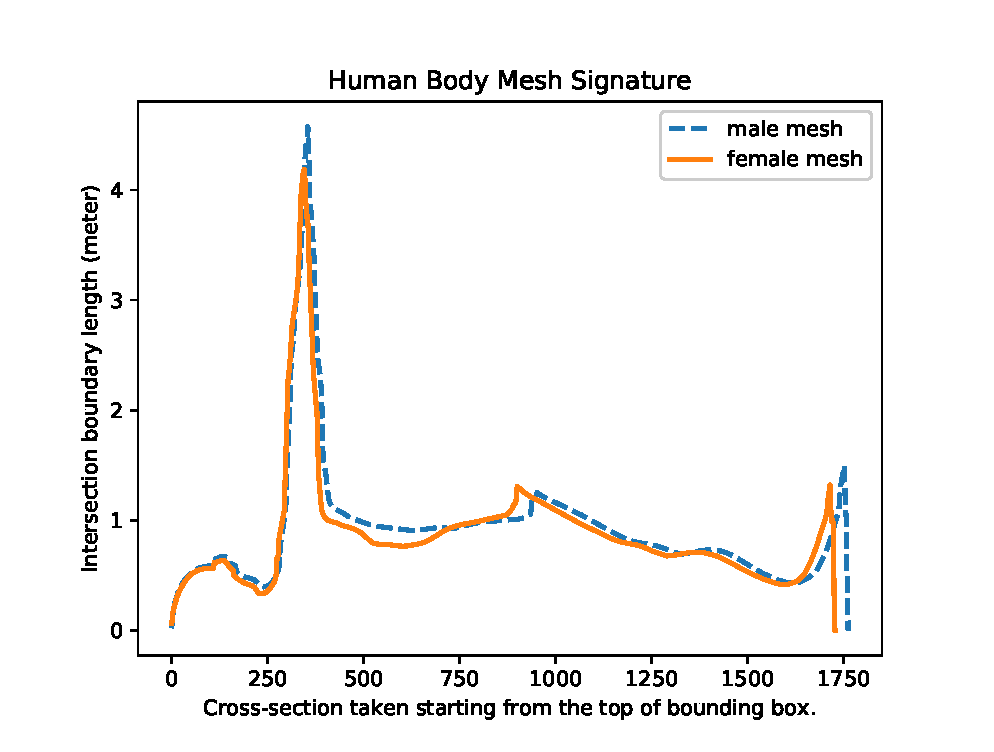
\includegraphics[width=\linewidth]{Figure_1.eps}
	\end{center}
	\caption{Human Body Mesh Signature for male and female meshes. The 
		function resembles a rotated silhouette of the human body and exhibits 
		several \textit{extrema}. See section 
		\ref{subsec:mesh_signature_extrema} for discussion of these extrema.}
	\label{fig:hbm_signature}
\end{figure}

Next, we assemble the mesh slide length vector $\vec{\mathcal{L}}$. Starting 
from the 
top $j_t$ of the bounding box we slice iteratively mesh $\mathcal{M}$ with 
plane 
$\boldsymbol{\pi_j}$ every $m$-meters until we reach the bounding box bottom 
$j_b$. Because the mesh $\mathcal{M}$ and the plane normal $\vec{n}_{||}$ 
remains the same we can drop them from the notation. For every slice at point 
$j$, we compute $\mathcal{BL}(j)$.

\begin{align}
\vec{\mathcal{L}}(\mathcal{M}, \vec{n}_{||}, m) = \left[ \mathcal{BL}(j_t), 
\mathcal{BL}(j_t+m), \cdots, \mathcal{BL}(j_b) \right]
\end{align}

Finally, we can define the human body \textbf{mesh signature} $\mathcal{MS}: 
\mathbb{Z}^+ \to \mathbb{R}$ that maps every slice index $k \in \{0, 1, \cdots, 
|\mathcal{L}|-1\}$ to the corresponding boundary length $\mathcal{BL}(j)$ in 
the mesh slide vector $\vec{\mathcal{L}}$.

\begin{align}\label{eq:mesh_signature}
\mathcal{MS}(k) = \mathcal{BL}(j)
\end{align}

Figure \ref{fig:hbm_signature} shows the $\mathcal{MS}$ of two meshes (male 
and female) for 
$m=0,001$ and plane $\boldsymbol{\pi}$ parallel to the floor (with normal $(0, 
1,0)$) using the library trimesh \cite{trimesh}. Note that the function as 
defined by equation \ref{eq:mesh_signature} is bounded and not continuous. It 
resembles a rotated silhouette of the human body and exhibits several 
\textit{extrema}.

In general, we expect these \textit{extrema} to be adequate features to 
calculate the human dimensions. However, there is no consensus in the 
literature regarding the method to calculate chest, waist and hip 
circumference. While Yansel et al., 2020 define waist circumference as the 
blalal. That is why we first establish the regions and the search for local 
extrema in these regions.

More specifically, we assume that:
\begin{enumerate}
	\item The global maximum $M_g$ represents the length of the largest path 
	around the arms. From a topographic point of view $M_g$ is the highest peak 
	of $\mathcal{MS}$. A horizontal line at height proportion $h$ of the peak 
	intersects 
	it at two points left $p_l$ and right $p_r$.
	\item The plane $\boldsymbol{\pi}$ intersects the mesh $\mathcal{M}$ at the 
	point where the left hip is located defining a path. The length of this 
	path is $P_{lh}$.	
	\item The local maximum $M_{pc}$ with largest value other than $M_g$ 
	immediately prior to $P_{lh}$ represents the pelvis circumference.	
	\item The local minimum $M_{wc}$ posterior to $p_r$ but prior to $M_{pc}$ 
	represents waist circumference.
	\item The local maximum $M_{cc}$ posterior to $p_r$ but prior to $M_{wc}$ 
	represents 
	chest circumference. If this local maximum does not exist we set $M_{cc}$ 
	to the value of the path $\mathcal{BL}(j_{cc})$ with largest value in the 
	interval $(p_l; M_{wc})$.
\end{enumerate}

\subsection{Recognition by interval search}\label{subsec:interval_search}

%------------------------------------------------------------------------
\section{Experiments and Results}

We conduct two experiments. In the first experiment we synthesize eight (four 
female and four male) human body meshes using shape parameters provided by 
SURREAL \cite{varol17_surreal}.
The meshes reflect human figures characteristics such as bulky, slim, small and 
tall subjects. Then we apply CALVIS to calculate chest, waist and pelvis 
circumference. Since we do not have ground truth, we evaluate the results 
qualitatively by comparing our method 
with \cite{Dibra.2016b}.
The second 
experiment serves to asses the plausibility of our approach to use the 
synthetic data for deep learning. We input the calculated human 
dimensions to an artificial neural network. After having trained the network 
with our data, we show that learning converges.

\subsection{Qualitative evaluation}\label{subsec:qualitative_eval}
Here we evaluate our method qualitatively with method one and method two.
\begin{figure}[H]
	\begin{center}
		%\fbox{\rule{0pt}{2in} \rule{0.9\linewidth}{0pt}}
		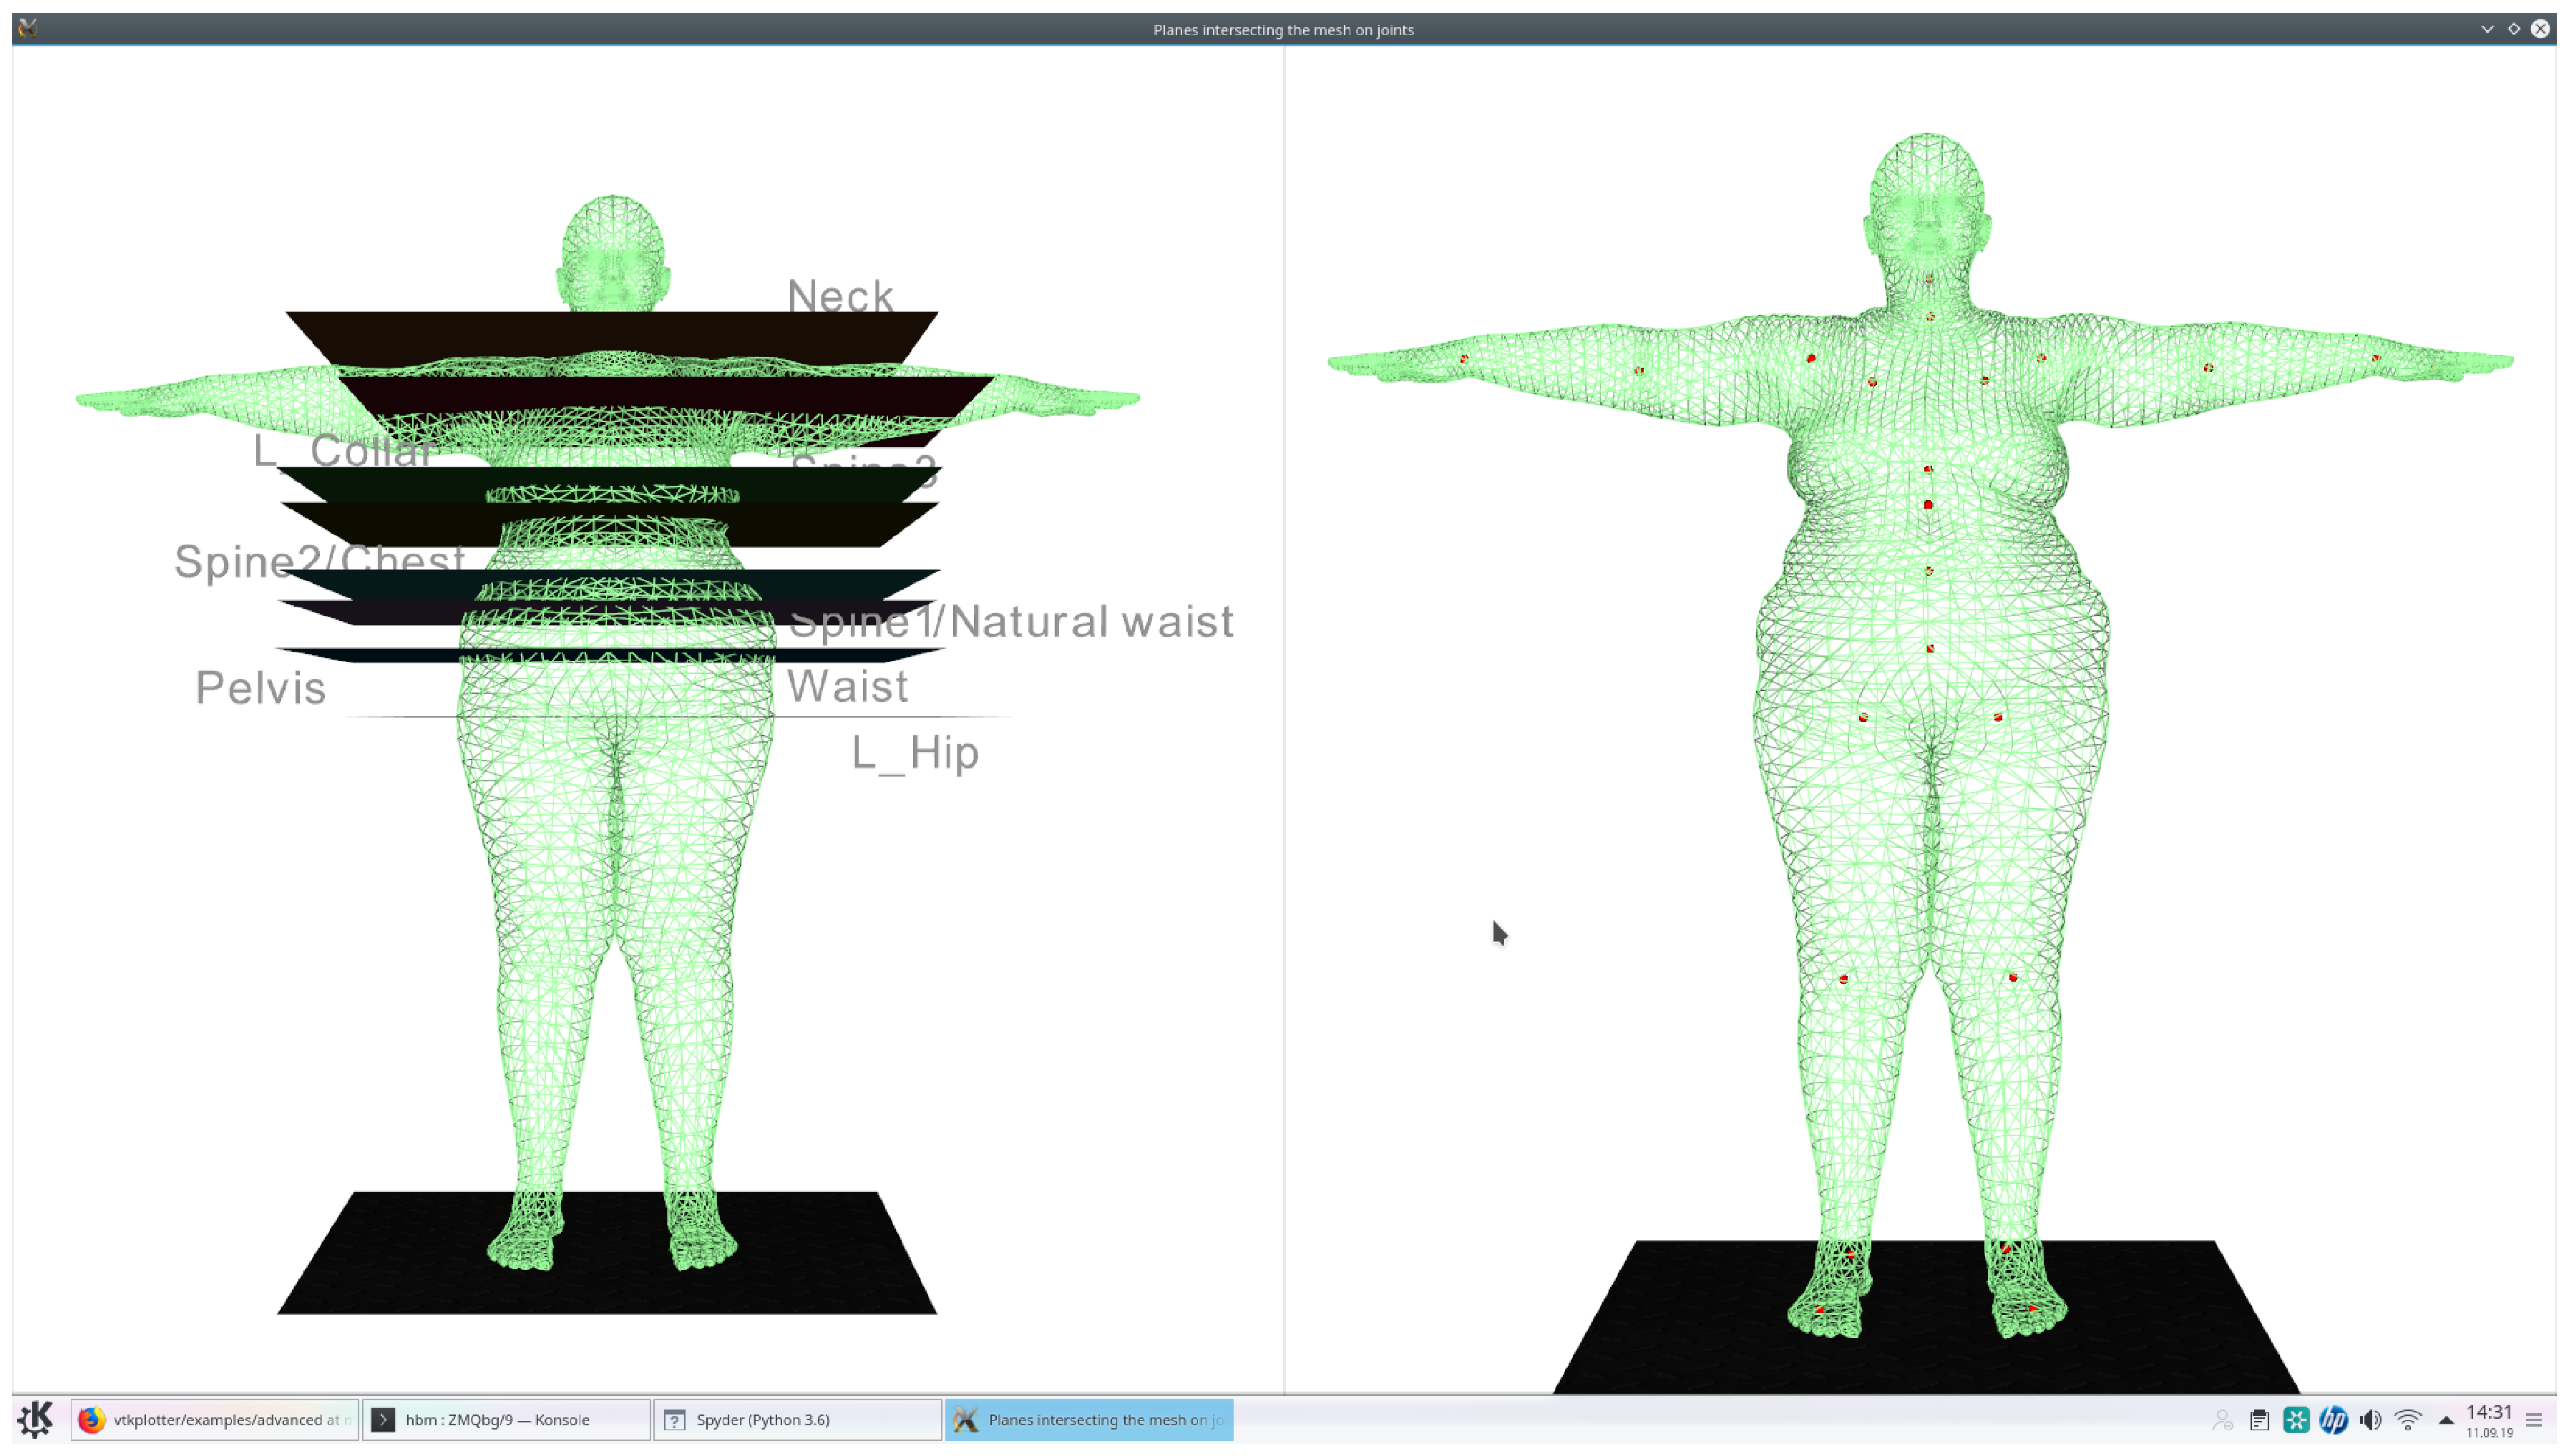
\includegraphics[width=\linewidth]{subject_6_with_cutting_planes_on_joints.eps}
	\end{center}
	\caption{Qualitative evaluation for male and female meshes. We evaluate our 
	method with method one and method two.}
	\label{fig:qualitative_eval}
\end{figure}

Figure \ref{fig:qualitative_eval} shows the $\mathcal{MS}$ of two meshes (male 
and female) for 
$m=0,001$ and plane $\boldsymbol{\pi}$ parallel to the floor (with normal $(0, 
1,0)$) using the library trimesh \cite{trimesh}. Note that the function as 
defined by equation \ref{eq:mesh_signature} is bounded and not continuous. It 
resembles a rotated silhouette of the human body and exhibits several 
\textit{extrema}.

\begin{figure}[h]
	\begin{center}
		%\fbox{\rule{0pt}{2in} \rule{0.9\linewidth}{0pt}}
		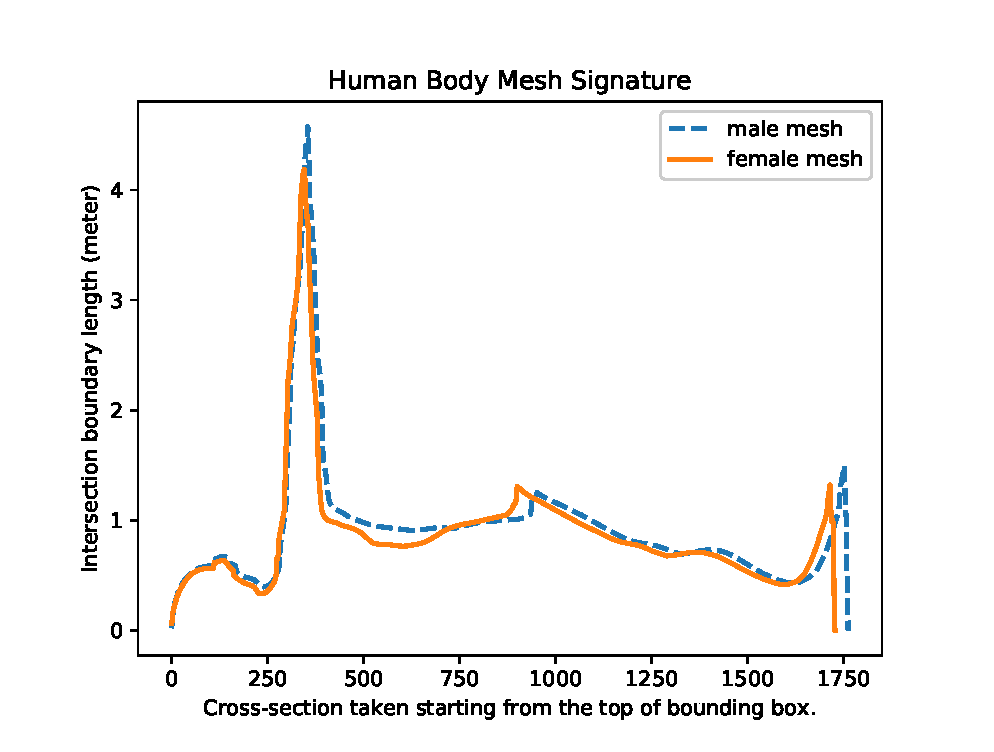
\includegraphics[width=\linewidth]{Figure_1.eps}
	\end{center}
	\caption{Human Body Mesh Signature for male and female meshes. The 
		function resembles a rotated silhouette of the human body and exhibits 
		several \textit{extrema}. See section 
		\ref{subsec:mesh_signature_extrema} for discussion of these extrema.}
	\label{fig:qualitative_eval}
\end{figure}

\subsection{Learning convergence evaluation}\label{subsec:learn_conv}
This experiment demonstrates the plausibility of using calvis to obtain data 
that can be used as a ground truth for machine learning (in general) and 
specifically as supervising signal for ANN.

Figure \ref{fig:calvis_net} shows the our prototypical ANN calvis net where the 
input is a synthetic image from a 3D mesh and the output are the three body 
dimensions.

Figure \ref{fig:learn_conv} shows that after epoch number 5 the estimation 
error decreases and the learning converges.

\begin{figure}[H]
	\begin{center}
		%\fbox{\rule{0pt}{2in} \rule{0.9\linewidth}{0pt}}
		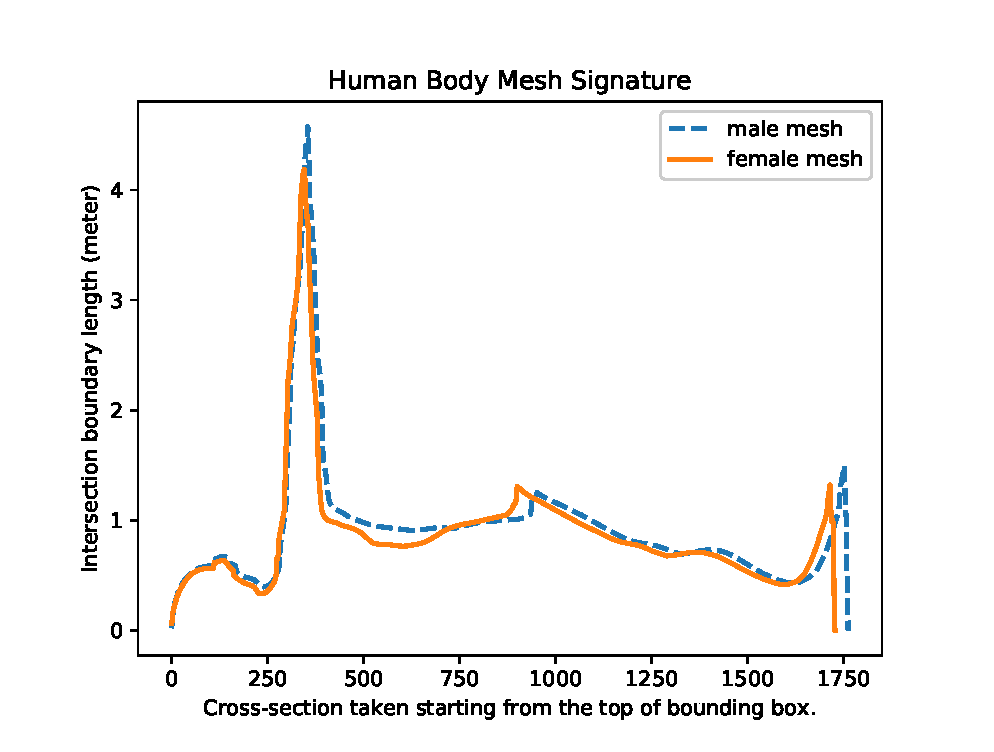
\includegraphics[width=\linewidth]{Figure_1.eps}
	\end{center}
	\caption{Human Body Mesh Signature for male and female meshes. The 
		function resembles a rotated silhouette of the human body and exhibits 
		several \textit{extrema}. See section 
		\ref{subsec:mesh_signature_extrema} for discussion of these extrema.}
	\label{fig:qualitative_eval}
\end{figure}

\begin{figure}[H]
	\begin{center}
		%\fbox{\rule{0pt}{2in} \rule{0.9\linewidth}{0pt}}
		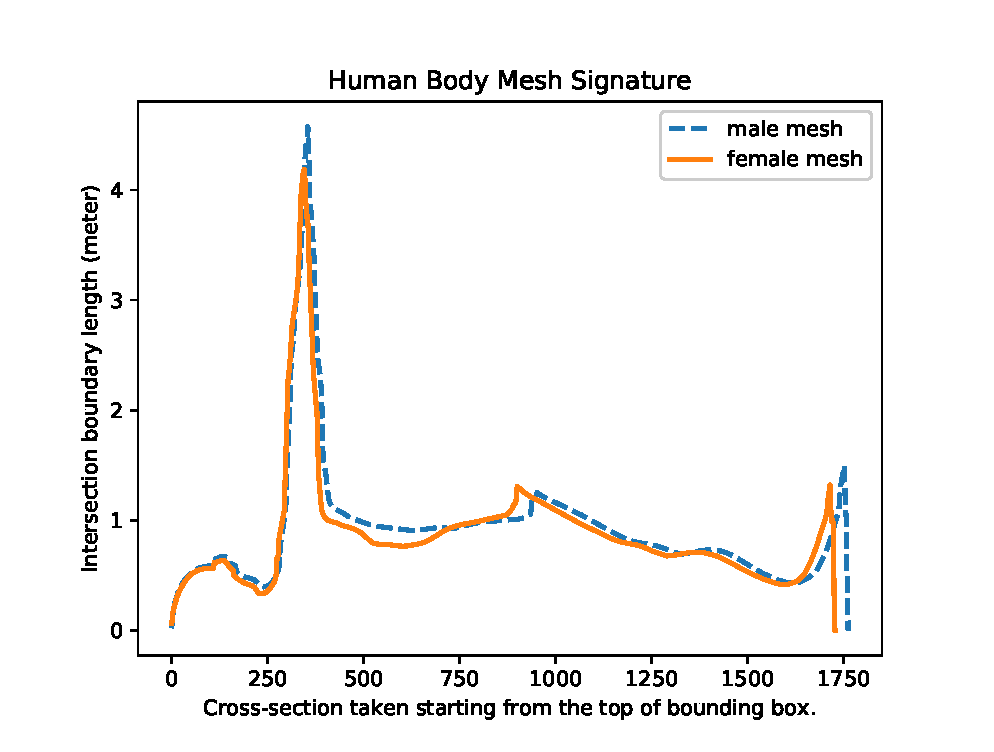
\includegraphics[width=\linewidth]{Figure_1.eps}
	\end{center}
	\caption{Human Body Mesh Signature for male and female meshes. The 
		function resembles a rotated silhouette of the human body and exhibits 
		several \textit{extrema}. See section 
		\ref{subsec:mesh_signature_extrema} for discussion of these extrema.}
	\label{fig:qualitative_eval}
\end{figure}


%------------------------------------------------------------------------
\section{Conclusion}

The method can be optimized. Further research must be conducted.
%
% ---- Bibliography ----
%
% BibTeX users should specify bibliography style 'splncs04'.
% References will then be sorted and formatted in the correct style.
%
\bibliographystyle{splncs04}
\bibliography{egbib}
%

\end{document}
